\chapter{Trabalhos Relacionados}
% ---
% ---esta seção, são exploradas pesquisas que compartilham afinidades e características semelhantes com os sistemas que este projeto busca desenvolver
Nesta seção, são exploradas pesquisas que compartilham afinidades e características semelhantes com o sistema que este projeto busca desenvolver.
   
\section{Aplicação \textit{WEB} Para Pessoas Físicas Que Utilizam Produtos Controlados Pelo Exército
Brasileiro E Polícia Federal}
A aplicação web denominada CRPG, tem o intuito de auxiliar os usuários a lidar com as etapas necessárias para a aquisição de produtos controlados pelo Exército Brasileiro e Polícia Federal. A \autoref{fig:grafico-crpg} demonstra a tela de cadastro de processos: 

\begin{figure}[htb]
    \caption{\label{fig:grafico-crpg}Tela de cadastros da aplicação CRPG}
    \begin{center}
        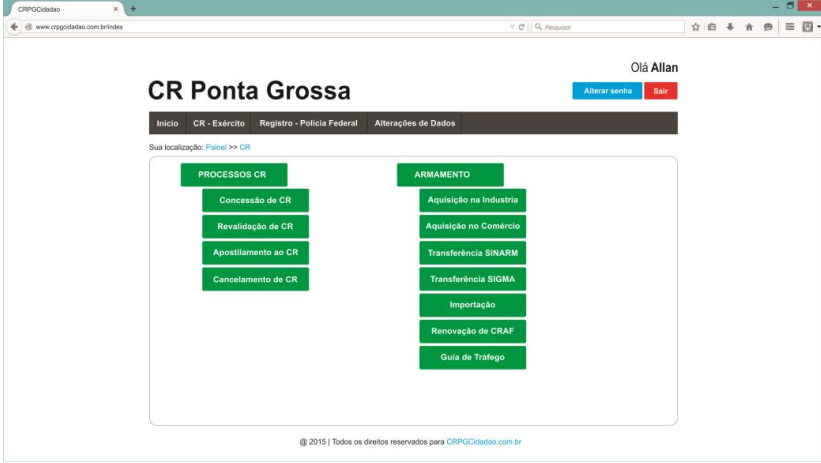
\includegraphics[scale=0.9]{imagens/crpg.png}
    \end{center}
    \legend{Fonte: \citeonline{crpg}}
\end{figure}

O Trabalho proposto se distingue da aplicação demonstrada acima, pois atua no âmbito de auxiliar os operadores da brigada militar afim de promover uma maior agilidade no processo de envio das informações para o SIGMA, buscando promover uma maior fluidez no controle e regulamentação dos produtos controlados sob jurisdição do exercito que estão sob posse destes indivíduos e entidades mencionadas na \autoref{sigmaesinarm}.



\section{Sistema De Gerenciamento De Licenças De Posse E Porte De Armas De Fogo}
Esta aplicação web se propõe a realizar todos os processos, como cadastro, validação de licenças, emissão de guias de tráfego, para indivíduos que tenham ou queiram adquirir o posse e porte de armas.
\url{https://sartori-ria.github.io/tcc-gun-licence-control-spa/}
\begin{figure}[htb]
    \caption{\label{fig:grafico-sglppa} Tela de cadastros da aplicação de Gerenciamento de Licenças}
    \begin{center}
        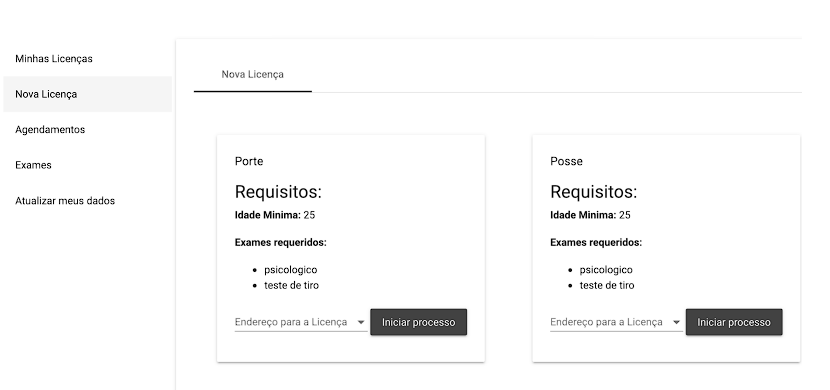
\includegraphics[scale=0.8]{imagens/sglppa.png}
    \end{center}
    \legend{Fonte: \citeonline{sglppa}}
\end{figure}

O presente trabalho destaca-se da aplicação anterior ao concentrar seus esforços na assistência aos operadores da brigada militar, visando agilizar o envio de informações para o SIGMA. A intenção é favorecer uma maior fluidez no controle e regulamentação desses produtos controlados sob jurisdição do exército.

\section{TAF- Teste de Aptidão Física da Brigada Militar do Rio Grande do Sul}
Um aplicativo móvel que visa facilitar a aplicação e avaliação do TAF na brigada militar do rio grande do sul. 
O TAF tem como objetivo verificar se os candidatos possuem as condições físicas mínimas exigidas para desempenhar as atividades do cargo \cite{taf}.

O aplicativo foi desenvolvido em parceria do IFRS com a BM RS, proporcionando mais projetos como este para alunos da instituição, trazendo benefícios para órgãos governamentais, fortalecendo a integração prática do conhecimento acadêmico com as demandas da sociedade.

Na \autoref{fig:grafico-taf} é demonstrado a tela inicial do TAF

\begin{figure}[htb]
    \caption{\label{fig:grafico-taf}Tela Inicial do aplicativo TAF BM}
    \begin{center}
        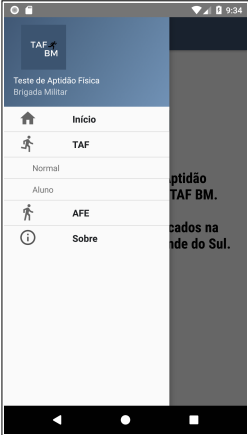
\includegraphics[scale=0.9]{imagens/taf.png}
    \end{center}
    \legend{Fonte: \citeonline{taf}}
\end{figure}
Por se tratar de resoluções em contextos diferentes, o aplicativo ''TAF'' se encaixa nesta seção por ter sido desenvolvido para a Brigada Militar do Rio Grande do Sul.